\documentclass[border=12pt]{standalone}
\usepackage{amsmath,amssymb}
\usepackage{pgfplots}
\pgfplotsset{compat=1.16}
\usepackage{booktabs}
\usepackage{array}
\begin{document}
\begin{minipage}{16cm}
\centering
{\large\bfseries Testable predictions: the $a_0=c^2\sqrt{\Lambda/32\pi}$ framework vs the major theories}\\[2pt]
{\footnotesize falsifiability $\star$ (effectively unfalsifiable near-term) to $\star\!\star\!\star\!\star\!\star$ (sharp, survived every test)}\\[10pt]
\begin{minipage}{7.4cm}
\small
\begin{tabular}{l c c l}
\toprule
Theory & Pred. & Confirmed & Falsif. \\
\midrule
QFT / Standard Model & $\sim$25 & nearly all & $\star\!\star\!\star\!\star\!\star$ \\
General relativity & $\sim$10 & all to date & $\star\!\star\!\star\!\star\!\star$ \\
$\Lambda$CDM & $\sim$9 & most & $\star\!\star\!\star\!\star$ \\
Cosmic inflation & $\sim$4 & spectrum & $\star\!\star\!\star$ \\
\textbf{This framework} & $\sim$9$^\dagger$ & RAR (shared) & $\star\!\star\!\star\!\star$ \\
Standard MOND & $\sim$8 & galaxy-scale & $\star\!\star\!\star\!\star$ \\
Verlinde emergent & $\sim$3 & mixed & $\star\!\star\!\star$ \\
Supersymmetry & $\sim$5 & none & $\star\!\star\!\star$ \\
Loop quantum gravity & $\sim$2 & none & $\star\!\star$ \\
String theory & $\sim$0 uniq. & none & $\star$ \\
\bottomrule
\end{tabular}\\[4pt]
{\scriptsize $^\dagger\sim$9 dated falsifiable; only $\sim$3 distinctive,\\ all from the $a_0(z)\!\propto\!\sqrt{\rho_{\rm DE}}$ spine.}
\end{minipage}\hfill
\begin{minipage}{8.0cm}
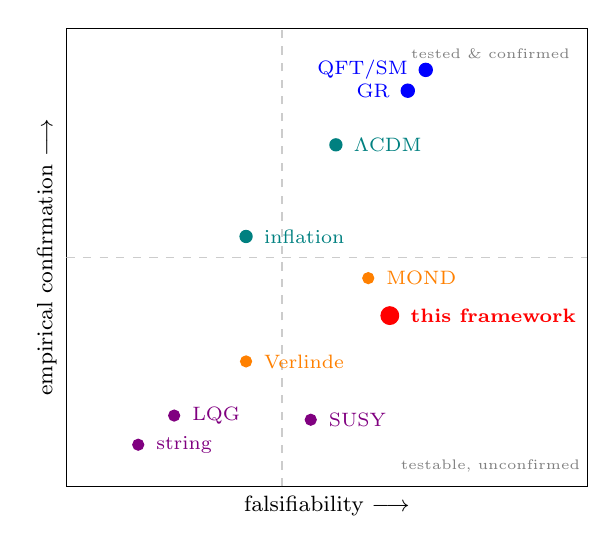
\begin{tikzpicture}
\begin{axis}[width=8.2cm,height=7.4cm,
  xlabel={falsifiability $\longrightarrow$}, ylabel={empirical confirmation $\longrightarrow$},
  xmin=0,xmax=14.5,ymin=0,ymax=11, xtick=\empty,ytick=\empty,
  grid=both, grid style={gray!15}, label style={font=\footnotesize}]
\addplot[only marks,mark=*,mark size=2.4pt,blue,nodes near coords,point meta=explicit symbolic,
  every node near coord/.append style={anchor=east,xshift=-3pt,font=\scriptsize}]
  coordinates {(10,10)[QFT/SM] (9.5,9.5)[GR]};
\addplot[only marks,mark=*,mark size=2.2pt,teal,nodes near coords,point meta=explicit symbolic,
  every node near coord/.append style={anchor=west,xshift=3pt,font=\scriptsize}]
  coordinates {(7.5,8.2)[$\Lambda$CDM] (5,6)[inflation]};
\addplot[only marks,mark=*,mark size=2.0pt,orange,nodes near coords,point meta=explicit symbolic,
  every node near coord/.append style={anchor=west,xshift=3pt,font=\scriptsize}]
  coordinates {(8.4,5.0)[MOND] (5,3)[Verlinde]};
\addplot[only marks,mark=*,mark size=2.0pt,violet,nodes near coords,point meta=explicit symbolic,
  every node near coord/.append style={anchor=west,xshift=3pt,font=\scriptsize}]
  coordinates {(6.8,1.6)[SUSY] (3,1.7)[LQG] (2,1.0)[string]};
\addplot[only marks,mark=*,mark size=3.2pt,red,nodes near coords,point meta=explicit symbolic,
  every node near coord/.append style={anchor=west,xshift=4pt,font=\scriptsize,red}]
  coordinates {(9,4.1)[\textbf{this framework}]};
\draw[gray!40,dashed] (axis cs:6,0)--(axis cs:6,11);
\draw[gray!40,dashed] (axis cs:0,5.5)--(axis cs:14.5,5.5);
\node[font=\tiny,gray] at (axis cs:11.8,10.4){tested \& confirmed};
\node[font=\tiny,gray] at (axis cs:11.8,0.5){testable, unconfirmed};
\end{axis}
\end{tikzpicture}
\end{minipage}
\end{minipage}
\end{document}
